\chapter*{Experiment 5 - Phenakistoscope Creation}
\addcontentsline{toc}{chapter}{Experiment 5 - Phenakistoscope Creation}
A Phenakistoscope is described as a spinning disc mounted on a handle which is mounted vertically. Printed on the disc is a series of images with a viewing slit cut into the disc in between each image. To use the Phenakistoscope, it is pointed towards a mirror, and the viewer looks through the slits. As the disc spins, the images blend together and an effect of movement is witnessed. It is possible to witness this same effect using a flashing LED in a dark room without the use of a mirror \citep{kalif-15-a} \citep{kalif-15-b} \cite{pepi-11}. For example images of Phenakistoscopes, see the examples on page:~\pageref{fig:phenakistoscopes}.

We wire up the experiment as shown in the diagram fig:~\ref{fig:exp5_phenakistoscope}. And upload the sketch code in the next section on page:~\pageref{sketch:exp5}.

%
\begin{figure}[ht]
	\centering
	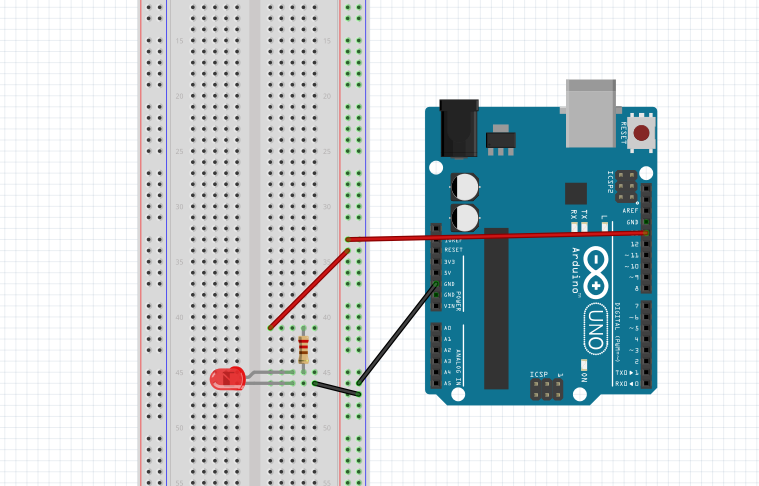
\includegraphics[width=12cm]{images/07}
	\caption{LED Phenakistoscope \citep{fritzing-15}}
	\label{fig:exp5_phenakistoscope}
\end{figure}
%

When the Arduino boots, the led should begin to flash repeatedly, on and off. When the \gls{Phenakistoscope} is spinning, the circuit can be used to light up and see the animation moving. This may require very low light conditions in order to see the effect clearly.

%
\begin{figure}
	\centering
	\begin{subfigure}[t]{5cm}
		\centering
		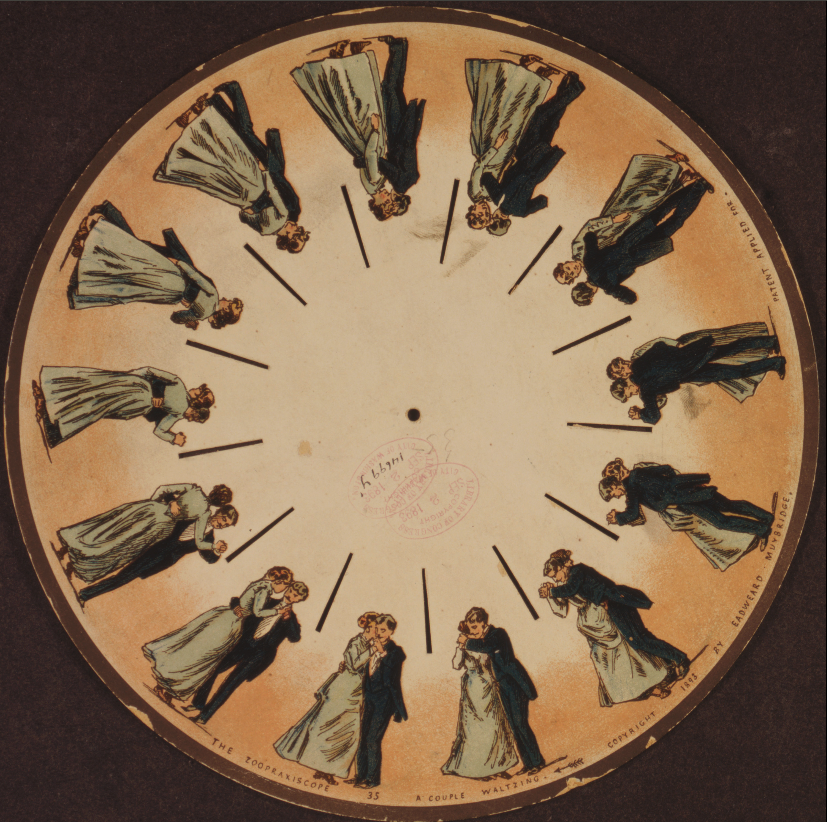
\includegraphics[width=5cm]{images/12}
		\caption{A couple waltzing - Eadweard Muybridge, 1893}
		\label{fig:gqrx_spectrogram_01} 
	\end{subfigure}
	\quad
	\begin{subfigure}[t]{5cm}
		\centering
		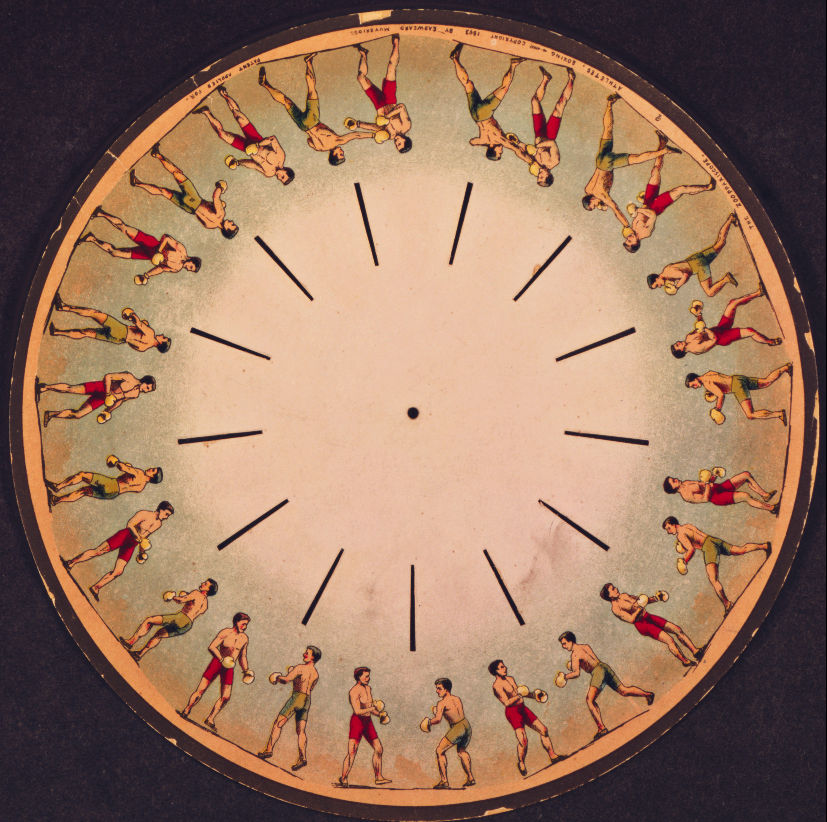
\includegraphics[width=5cm]{images/13}
		\caption{Athletes Boxing - Eadweard Muybridge, 1890}
		\label{fig:rtl_power_spectrogram_01} 
	\end{subfigure}
	\quad
	\begin{subfigure}[t]{5cm}
		\centering
		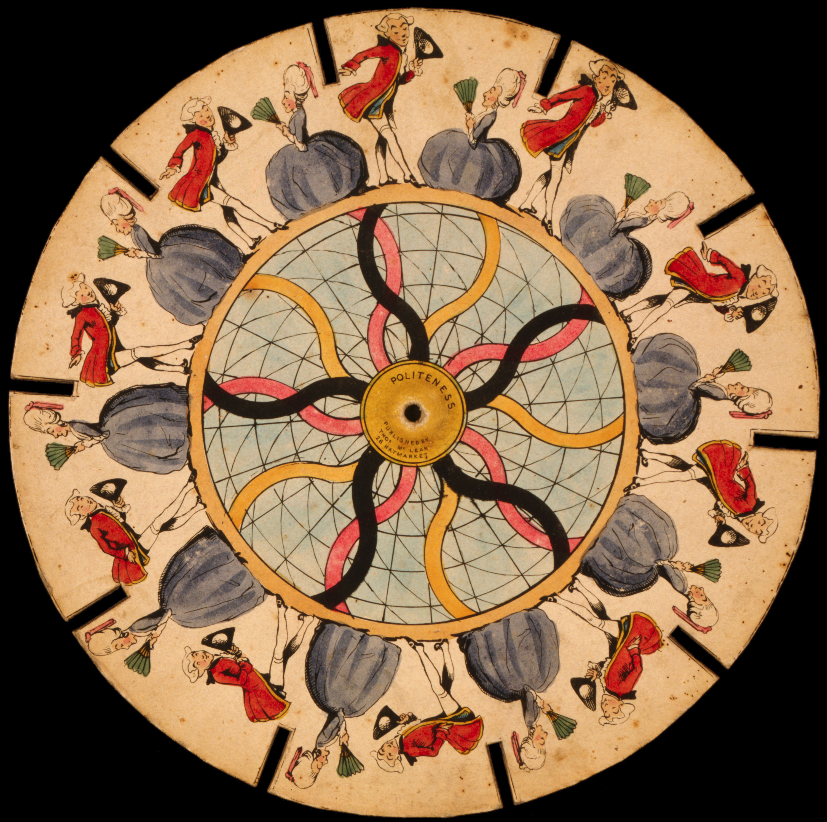
\includegraphics[width=5cm]{images/14}
		\caption{Politeness - Thos. McLean, 1833}
		\label{fig:rtl_power_spectrogram_02} 
	\end{subfigure}
	\quad
	\begin{subfigure}[t]{5cm}
		\centering
		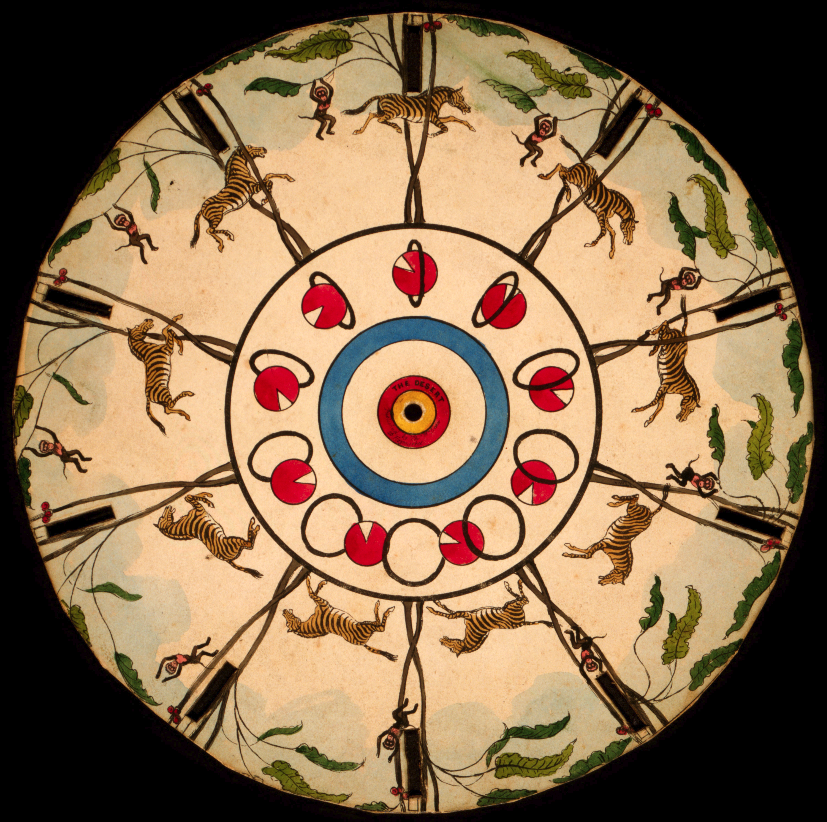
\includegraphics[width=5cm]{images/15}
		\caption{The Desert - Thos. McLean, 1833}
		\label{fig:rtl_power_spectrogram_03} 
	\end{subfigure}
	\quad
	\caption{A selection of Phenakistoscopes}
	\label{fig:phenakistoscopes}
\end{figure}
%


\newpage
\section*{Sketch Code}
\label{sketch:exp5}
\begin{lstlisting}
/*
Phenakistoscope
Turns on an LED on then off 20 times a second in order to activate the Phenakistoscope
*/

// the setup function runs once when you press reset or power the board
void setup() {
  // initialize digital pin 13 as an output.
  pinMode(13, OUTPUT);
}

// the loop function runs over and over again forever
void loop() {
  // turn the LED on 
  // (HIGH is the voltage level)
  digitalWrite(13, HIGH);
	
  //wait for 10 milliseconds
  delay(10);
	
  // turn the LED off by making 
  // the voltage LOW
  digitalWrite(13, LOW);    
	            
  // wait for 30 milliseconds              
  delay(30);
}
\end{lstlisting}